\documentclass[a4paper,12pt]{report}

\usepackage{alltt, fancyvrb, url}
\usepackage{authblk}
\usepackage{graphicx}
\usepackage{subfigure}
\usepackage{wrapfig}
\usepackage{algorithmic}
\usepackage[utf8]{inputenc}
\usepackage{fontenc}
\usepackage{amsmath,stmaryrd,mathtools,algorithm}
\usepackage{amssymb}
\usepackage[document]{ragged2e}
\usepackage[italian]{babel}

\title{\Huge \textbf{Relazione Progetto OOP}}
 
\author{Giulianini Andrea, Lombardi Alessandro, Meluzzi Marco, Stockman Alessandro}
\date{\today}


\begin{document}
 
\maketitle
\justify

\tableofcontents

\chapter{Analisi}

\section{Requisiti}

Il programma qbert è un remake del videogioco arcade Q*Bert pubblicato nel 1982 dalla  Gottlieb. In altri termini si tratta di un rifacimento che  tende a ricostruire abbastanza  fedelmente, se non tutte, almeno le principali caratteristiche del gioco originale.

\subsubsection{Requisiti funzionali}
\begin{itemize}
	\item Il giocatore servendosi degli appositi input da tastiera, può muovere il personaggio principale in quattro direzioni. Lo scopo di ogni round, con i quali si articola il gioco, è colorare gradualmente la faccia superiore di ciascun cubo della mappa piramidale di un certo colore.
	\item Il numero di colori e i colori stessi che un cubo può assumere possono variare da un livello all'altro. Esiste inoltre la possibilità di ricominciare a ciclare il set colori disponibili una volta raggiunto l'ultimo, rendendo di fatto più complesso l'obiettivo del gioco.
	\item Nel gioco sono presenti vari personaggi, l'interazione fra il protagonista e questi avviene tramite contatto, alcuni di questi sono amici, quindi possono favorire il protagonista nel raggiungimento del suo obiettivo, altri sono nemici. Generalmente i nemici sono da evitare, in quanto una collisione con questi sarebbe letale per il protagonista, ma vi sono altri che possono essere eliminati. I personaggi possono avere movimenti e comportamenti differenti.
	\item I movimenti possono andare dall'alto verso il basso, terminando a seconda del personaggio specifico con una caduta fuori dalla mappa oppure con movimenti più intelligenti e tendenti ad inseguire il giocatore.
	\item Dal punto di vista dell’ambiente di gioco, questo deve adattarsi consistentemente all’avanzamento dello stesso, in modo da rispecchiare la struttura a livelli prevista e il graduale aumento della difficoltà del gameplay.
	\item Il vero scopo del giocatore è sopravvivere e ottenere punteggi elevati. E' possibile guadagnare punti in diversi modi durante il corso della partita.
\end{itemize}

\subsubsection{Requisiti non funzionali}
\begin{itemize}
	\item Realizzazione di una grafica molto simile a quella originale ma più moderna
	\item Garantire la fluidità dell’esperienza di gioco

\end{itemize}

\section{Analisi e modello del dominio}

Il programma deve gestire una sessione di gioco composta da vari livelli, certe informazioni si mantengono da un livello all'altro, ad esempio le vite del protagonista oppure il punteggio accumulato, mentre altre saranno ogni volta ricalcolate. Un livello presenta elementi "statici", come la natura dei cubi di cui è composto, e "dinamici", come il set di antagonisti che si possono incontrare. Il livello si occupa della creazione e aggiornamento del terreno di gioco gestendo gli oggetti statici presenti,  dell'aggiornamento del punteggio causato da differenti eventi e del controllo della corretta esecuzione delle regole del gioco. Il livello interagisce con un'altra entità, detta Spawner, per controllare che la quantità dei personaggi in azione sia adatta al livello di difficoltà raggiunto. Il ciclo di vita dei personaggi è spesso breve e semplice, essi eseguono una serie di movimenti personalizzati e indipendenti, mentre interagiscono con l'ambiente esterno quasi univocamente tramite collisione.

Fra le difficoltà che si potrebbero incontrare potrebbe esserci quella di costruire un dialogo livello-personaggi-spawner in modo da mantenere una certa indipendenza tra le entità e una suddivisione chiara dei ruoli. Il requisito non funzionale sulla giocabilità del software finale richiederà molte prove e una certa dose di abilità di game design, quindi sarà fatto verso la fine e potrà essere accorciato per motivi di tempo.

\begin{figure}[H]
\centering{}
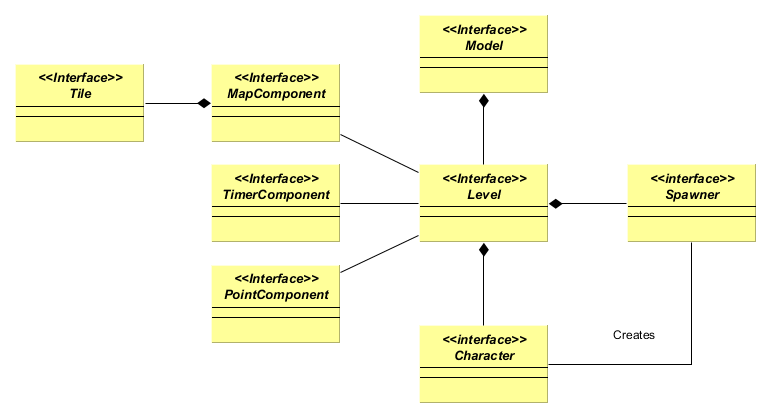
\includegraphics[width=\linewidth]{img/Analisi}
\caption{Schema dell'analisi e modello del dominio}
\label{img:Analysis}
\end{figure}

\chapter{Design}

\section{Architettura}

L'architettura dell'applicazione è realizzata utilizzando il pattern architetturale MVC in quanto permette facilmente di separare la logica e i dati della applicazione dalla effettiva tecnica adottata per la visualizzazione di questi. La applicazione e la relativa architettura può essere spezzata in varie implementazioni associate allo stato nella quale si trova attualmente.

L'interfaccia Model fornisce tutte le funzionalità comuni ad ogni fase della applicazione per comunicare al Controller i dati da mostrare e presentare i comandi in grado di influenzare l'esecuzione della logica interna. La gestione dello stato corrente e la relativa implementazione lato model è fatta da una entità preposta del Controller detta GameStatusManager. 

\begin{figure}[H]
\centering{}
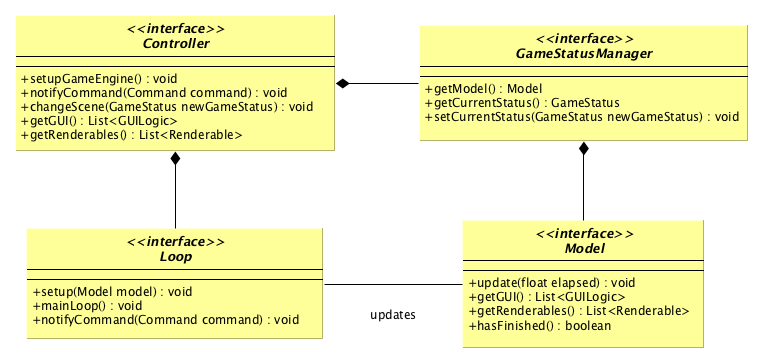
\includegraphics[width=\linewidth]{img/ArchitetturaControllerModel}
\caption{Il dialogo fra Controller e Model}
\label{img:ControllerModel}
\end{figure}

Il Controller si occupa principalmente di gestire il dialogo fra Model e View, oltre che di fornire numerose funzionalità per la lettura e scrittura su file di diversi tipi di dati persistenti. Il Controller deve inoltre gestire una componente vitale della applicazione detta Loop, che permette di aggiornare grafica e logica nel tempo, sostituendo in pratica gli elementi da aggiornare quando cambia lo stato del programma.

Il dialogo fra Controller e View è più stabile in quanto è la View stessa ad associare a differenti scene lo stato di gioco e di realizzare effettivamente il cambio da una scena all'altra. Scene svolge effettivamente la renderizzazione grafica sfruttando particolari classi che aggiorna il Model e che confezionano tutte le informazioni necessarie per disegnare correttamente immagini (Renderable) e GUI (GUILogic).

\begin{figure}[H]
\centering{}
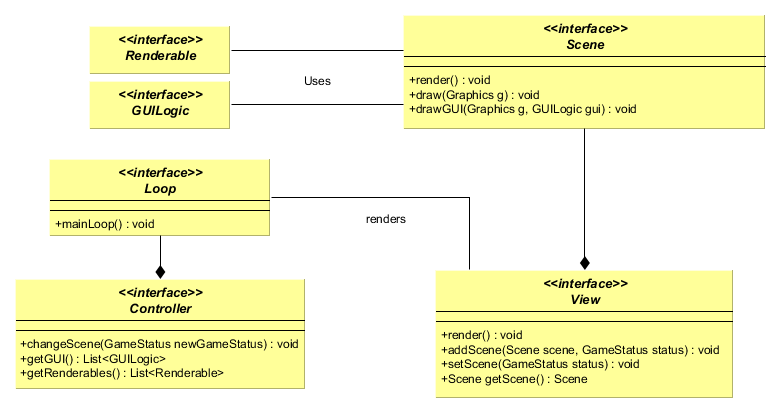
\includegraphics[width=\linewidth]{img/ArchitetturaControllerView}
\caption{Il dialogo fra Controller e View}
\label{img:ControllerView}
\end{figure}

\section{Design dettagliato}


\chapter{Sviluppo}
\section{Testing automatizzato}


\section{Metodologia di lavoro}


\section{Note di sviluppo}


\chapter{Commenti finali}


\section{Autovalutazione e lavori futuri}


\section{Difficoltà incontrate e commenti per i docenti}


\appendix
\chapter{Guida utente}


%\bibliographystyle{abbrv}
%\bibliography{template}

\end{document}